  %%%%%%%%%%%%%%%%%%%%%%%%%%%%%%%%%%%%%%%%%%%%%%%%%%%%%%%%%%%%%%%%%%%%%%
% LaTeX Example: Project Report

%%% Preamble
\documentclass[paper=a4, fontsize=11pt, abstract=on]{scrartcl}
\usepackage[T1]{fontenc}
\usepackage{fourier}
\usepackage{tabularx}
\usepackage[utf8]{inputenc}
\usepackage{hyperref}





\usepackage{listings}
\usepackage{color}

\definecolor{dkgreen}{rgb}{0,0.6,0}
\definecolor{gray}{rgb}{0.5,0.5,0.5}
\definecolor{mauve}{rgb}{0.58,0,0.82}
\lstset{frame=tb,
  language=[Visual]C++,
  aboveskip=3mm,
  belowskip=3mm,
  showstringspaces=false,
  columns=flexible,
  basicstyle={\small\ttfamily},
  numbers=none,
  numberstyle=\tiny\color{gray},
  keywordstyle=\color{blue},
  commentstyle=\color{dkgreen},
  stringstyle=\color{mauve},
  breaklines=true,
  breakatwhitespace=true,
  tabsize=3
}
\usepackage{graphicx}
\usepackage{caption}
\usepackage{subcaption}

\usepackage[english]{babel}															% English language/hyphenation
\usepackage[protrusion=true,expansion=true]{microtype}	
\usepackage{amsmath,amsfonts,amsthm} % Math packages

\usepackage{url}
%\usepackage[hang, small,labelfont=bf,up,textfont=it,up]{caption}


%%% Custom sectioning
\usepackage{sectsty}
\allsectionsfont{\normalfont\scshape}
\usepackage{float}
\usepackage{amsmath}
\usepackage{mathtools}
\usepackage{ragged2e}

\usepackage{nomencl}
\makenomenclature

%%% Custom headers/footers (fancyhdr package)
\usepackage{fancyhdr}
\pagestyle{fancyplain}
\fancyhead{}											% No page header
\fancyfoot[L]{}											% Empty 
\fancyfoot[C]{}											% Empty
\fancyfoot[R]{\thepage}									% Pagenumbering
\renewcommand{\headrulewidth}{0pt}			% Remove header underlines
\renewcommand{\footrulewidth}{0pt}				% Remove footer underlines
\setlength{\headheight}{13.6pt}
   \renewcommand*\abstractname{Summary}

%%% Equation and float numbering
\numberwithin{equation}{section}		% Equationnumbering: section.eq#
\numberwithin{figure}{section}			% Figurenumbering: section.fig#
\numberwithin{table}{section}				% Tablenumbering: section.tab#


%%% Maketitle metadata

\newcommand{\horrule}[1]{\rule{\linewidth}{#1}} 	% Horizontal rule

\title{
		%\vspace{-1in} 	
		\usefont{OT1}{bch}{b}{n}
		\normalfont \normalsize \textsc{} \\ [25pt]
		
\includegraphics[width=0.3\linewidth]{ubc.png} \\
		%
\includegraphics[width=0.4\linewidth]{tru}		
		\horrule{0.5pt} \\[0.2cm]
		\huge Programming Assignment \#2 : Solving 1D Wave Equation  \\
		\horrule{2pt} \\[0.005cm]
}
\author{
		\normalfont 								\normalsize
        Jerin Roberts\\[-5pt]		\normalsize
        \today
}
\date{}




%%% Begin document
\begin{document}
\maketitle
\begin{center}
\begin{tabular}{l r}


Supervisor: & Dr. Carl Ollivier-Gooch  \\ % supervisor
Locations: & University of British Columbia


\end{tabular}
\end{center}



\newpage
\tableofcontents
\listoffigures
\listoftables
\newpage
\lstset{language=[Visual]C++}
\section{Overview}



 The are many physical phenomenons in physics and engineering that require linear and non-linear partial differential equations to described the true nature of the system. Solving these systems analytically and finding exact solutions for these equations can be difficult and often require simplifications that ultimately don't fully represent the problem being investigated. Numerical methods for solving PDE's provides a means of finding approximations to the exact solutions without having to make sacrificial simplifications. With recent advancements in computational technology numerical methods can now be easily applied to large and difficult problems that would otherwise be impossible to solve. 
\subsection{Theory}
Numerical problems are essentially solved by breaking the entire solution domain into small discrete points (mesh) and finding the solution at or around these areas. Each point requires the solving the differential equations that represent physical phenomenon being investigated. Since the exact solution cannot be computed, it is instead approximated using various techniques and methods. 

The Runge-Kutta scheme is a family of numerical techniques used to solve ordinary differential equations by numerically integrating using trial steps at the midpoints of an interval to cancel out lower-order error terms. A two stage Runge-Kutta scheme is displayed in equation \ref{rung2} which uses Explicit Euler as the first stage intermediate step \ref{rung1}.
 

 \begin{equation}
\label{rung1}
w^{(1)}=w^n+\triangle t(\lambda w^n)
\end{equation} 


 \begin{equation}
\label{rung2}
w^{n+1}=w^n+\triangle t\Bigg(\frac{\lambda w^n+\lambda w^{(1)}}{2}\Bigg)
\end{equation}

 The program will implement a 2nd order up wind flux evaluation method and a two-stage Runge-Kutta time advance scheme. For each interior volume cell the net flux will be calculated for a specific time step using the second order up wind method. The flux for the face $i=3/2$ is displayed in equation \ref{fl}. The flux is evaluated at each face and then the faces surrounding a single cell are summed to find the flux through that cell. Integrating this into equation \ref{wave} the wave equation can be evaluated using equation \ref{th}

 \begin{equation}
\label{fl}
T_{\frac{3}{2}}=\frac{3\overline{T}_{1}-\overline{T}_{0}}{2} 
\end{equation}

 \begin{equation}
\label{th}
\frac{\partial T}{\partial t} + u\Bigg(\frac{3\overline{T}_{i}-4\overline{T}_{i-1}+\overline{T}_{i-2}}{2\triangle x}\Bigg)  = 0
\end{equation}

Boundary conditions will be implement using ghost cells allowing the interior scheme to remain the same during calculation of bordering cells. Because the interior scheme requires two upwind values, two ghost cells are required for this scheme to run on the first interior cell $i=1$. The ghost cells are calculated such the boundary condition is enforced at $i=1/2$. 



\begin{equation}
\label{neum}
\overline{T}_{0} = 2\overline{T}_{w}-\overline{T}_{1} 
\end{equation} 

\begin{equation}
\label{neum2}
\overline{T}_{-1} = -2\overline{T}_{w}+3\overline{T}_{0} 
\end{equation} 


The value for the ghost cells implementing Neumann Boundary at $x=0$ is calculated using equation \ref{neum} for cell $i = 0$ and \ref{neum2} for cell $i = -1$.
 


\section{Implementation}
\subsection{Program Overview}
The C/C++language was selected for this programming assignment. The scripts were compiled using g++/gcc version 5.4.0 on Ubuntu 16.04.02 and are available in the attached zip or for clone via the link provided: \url{https://github.com/j16out/cfd510} . The program itself is broken into 3 pieces and two levels to produce a modular set that makes it easier to apply to different problems. The highest level contains the "macro" or the main function which can be modified for different problems. The numerical directory contains numerical.cpp script and its header file numerical.hpp. This set contains all the functions necessary for solving the problem numerically. Table \ref{func} displays all functions with a short description of each. The vroot directory contains the scripts necessary for drawing data. These scripts make use of the ROOT-v6 libraries. ROOT is a popular data analysis framework primarily written in C++ and Phython. For more information on ROOT libraries visit the link provided: \url{https://root.cern.ch/} .

\begin{table}[H]
\begin{center}
    \begin{tabular}{ | p{0.21\linewidth} | p{0.6\linewidth} |}
 \hline  
     \RaggedRight \textbf{Function}
    &\RaggedRight \textbf{Purpose}
    \\ \hline  
           \RaggedRight set\_ array\_ size() 
    &\RaggedRight Set size of array if not default(160x160)
    \\ \hline 
           \RaggedRight set\_ ghostcells()
    &\RaggedRight Set Ghost cells and update boundary conditions
    \\ \hline 
           \RaggedRight set\_ zero()
    &\RaggedRight Zero entire array including ghost cells
    \\ \hline 
           \RaggedRight print\_ array()
    &\RaggedRight Prints array in terminal style output
    \\ \hline 
           \RaggedRight gs\_ iter\_ SOR() 
    &\RaggedRight Performs single Gauss-Seidel iteration with over-relaxation, over first in y then x
    \\ \hline 
           \RaggedRight calc\_ source()
    &\RaggedRight Calculates the source term for the problem
    \\ \hline 
      \RaggedRight calc\_ newcell()
    &\RaggedRight Calculates new solution at single grid point
    \\ \hline 
    \RaggedRight  get\_ surcells()
    &\RaggedRight Gets current solution of neighboring cells
    \\ \hline 
    \RaggedRight solve\_ arraySOR()
    &\RaggedRight Solves for solution by performing many GS-iterations until defined convergence is met
    \\ \hline 
    \RaggedRight get\_ discrete\_ Error()
    &\RaggedRight Returns error for solution at P(1/2,1/2) for Poisson Problem
    \\ \hline 
    \RaggedRight get\_ solution()
    &\RaggedRight Returns Solution at P(1/2,1/2) for Poisson Problem via averaging scheme
      \\ \hline 
    \RaggedRight get\_ l2norm()
    &\RaggedRight Returns $L^2$ norm error between two arrays of equal size
    \\ \hline 
    \RaggedRight set\_ analytic() 
    &\RaggedRight Set array values to predefined exact solution
    \\ \hline 
    
    
    \end{tabular}
\end{center} 
\caption{List of Program Functions}
\label{func} 
\end{table}

The functions act on a structure called $carray$ which contains the solution domain array and its various parameters. The Struct contains the main array, its defined working area (mesh size), data storage vectors, iteration count, and the represented dimension between points. Having these organized in a struct provides a compact way of passing and modifying the array and all its pertinent parameters. The outline of the struct used for the wave equation problem is shown below.


\begin{lstlisting}
struct carray{
//arrays
float mcellSOL [maxx][maxy];//first stage and solution mesh
float mcellSOL2 [maxx][maxy];//second stage solution mesh
float mcellFI [maxx][maxy];//first stage flux
float mcellFI2 [maxx][maxy];//second stage flux

//array attributes
int sizex = maxx;
int sizey = maxy;
float DIM1 = 0;

//current time 
float tstep = 0;
float ctime = 0;

//temporary cells to store
float Tim1_j=0.0;
float Tim2_j=0.0;
float Ti_j=0.0;

};
\end{lstlisting}
 
\subsection{1D Wave Problem}
The program was used to solve and find solutions to the 1D wave equation with information moving left to right (\ref{sim}) with satisfying conditions (\ref{con}). An exact solution to this problem is provided and written as $T(x,t)$ and displayed in equation \ref{ddd} which will enabled a comparison for solution error assessment. 

 \begin{equation}
\label{sim}
\frac{\partial T}{\partial t} + u\frac{\partial T}{\partial x} = 0
\end{equation}

 \begin{equation}
\label{con}
0\leq x \leq x_{max} \hspace{35pt} 0 \leq t \hspace{35pt} u = 2
\end{equation}

 \begin{equation}
\label{ddd}
T(x,t) = \sin{(2\pi (2t-x))}
\end{equation}

\subsection{Boundary Conditions}
Boundary Conditions are implemented through the calculation of the ghost cells. For the purely up wind scheme, we require two ghost cells to be calculated. The ghost cell is calculated such that the boundary is implemented at the face between the first ghost cell and first border cell. Below shows the function that implements boundaries for the Wave problem.

\begin{lstlisting}
void set_ghostcells(carray & myarray)
{
//set boundary conditions in ghost cells
myarray.mcellSOL2[0][1] = -2.0*(sin(4.0*PI*myarray.ctime)) + 3.0*myarray.mcellSOL[1][1];
myarray.mcellSOL2[1][1] = 2.0*(sin(4.0*PI*myarray.ctime)) - myarray.mcellSOL[2][1];	
}
\end{lstlisting}
A loop is not necessary as this is purely a 1D problem therefore only two cells need to be updated each time step iteration. This subroutine will need to be modified when the program is applied to different problems or using different flux schemes at the boundary. At this stage is not changeable during run-time. Initial Conditions are set before the problem is solved using the subroutine shown below.
\begin{lstlisting}
void set_intial_cond(carray & myarray)
{
float DIM1 = myarray.DIM1;
float dx =0.0;
float f;
for(int j = 1; j < myarray.sizey-1; ++j)
{
    for(int i = 2; i < myarray.sizex; ++i)
    {
    dx = (i-1.5)*DIM1;
    f = -sin(2.0*PI*dx);
    myarray.mcellSOL[i][j] = f;
    }
}
}
\end{lstlisting}
The loop calculates all the values of T at time t=0 for varying x using equation \ref{int}. Similar to the boundary conditions the initial conditions are not modifiable during run-time and will need to be tailored to specific problems.

 \begin{equation}
\label{int}
T(x,0) = -\sin{(2\pi x)}
\end{equation}
  
\subsection{Iteration Scheme}
A RK2 routine was implemented to solve the system of equations approximating the solution at each grid point which is denoted as function $solve\_ arrayRK2$. The routine starts from the first interior cell $i = 2$ and iterates flux integration schemes until $i = i_{max}$. Once the flux values have been gathered for each face and expressed as a single cell value a subroutine calculates the time advance solution at each cell. Below shows both the flux calculating and solution calculating subroutines respectively.

\begin{lstlisting}
void get_FIarray(carray & myarray, int stage)
{
for(int j = 1; j < myarray.sizey-1; ++j)
{
    for(int i = 3; i < myarray.sizex; ++i)
    {
    //----get surrounding cells and compute new cell-------//
    get_surcells(myarray, i, j, stage);
    float newcell = calc_2nd_UW(myarray); 
    //-----update current cell----//
    if(stage == 1)
    myarray.mcellFI[i][j] = newcell;
    if(stage == 2)
    myarray.mcellFI2[i][j] = newcell;
    }
}
}
\end{lstlisting}
\begin{lstlisting}
void get_RK2(carray & myarray, int stage)
{
if(stage == 1)
{
for(int j = 1; j < myarray.sizey-1; ++j)
{
    for(int i = 2; i < myarray.sizex; ++i)
    {
      myarray.mcellSOL2[i][j] = myarray.mcellSOL[i][j]-myarray.tstep*(myarray.mcellFI[i][j]);
    }
}
}
if(stage == 2)
{
for(int j = 1; j < myarray.sizey-1; ++j)
{
    for(int i = 2; i < myarray.sizex; ++i)
    {
     myarray.mcellSOL2[i][j] = myarray.mcellSOL[i][j]-myarray.tstep*((myarray.mcellFI2[i][j]+myarray.mcellFI[i][j])/2.0);
    }
}
}
}
\end{lstlisting}

It should be noted the first interior cell i = 2 flux is calculated in a seperate sub routine called $get\_ FIarray\_ 1stcell$.
An outer solving loop implements the RK2 scheme via two stages for all required time steps. After the two stages are computed the scheme is advanced by one time step and the boundary conditions are re-evaluated and implemented by calculating the new ghost cell values for the latest solution. Below displays the solution solving loop:
\begin{lstlisting}
void solve_arrayRK2(carray & myarray, float tmax, float cfl)
{
float tstep = (cfl*(myarray.DIM1))/2.0;
myarray.tstep = tstep;
float ctime = myarray.ctime;

//set intial conditions
set_intial_cond(myarray);
set_ghostcells(myarray);

  while(ctime < tmax-tstep)
  {
  
   for(int h = 1; h <= 2; ++h)
    { 
    get_FIarray_1stcell(myarray, h);//(array, stage)
    get_FIarray(myarray, h);//(array, stage)
    get_RK2(myarray, h);//(array, stage)
    }

  //mv sol2 back to array sol1
  mv_SOL2_to_SOL1(myarray);

  //flux at boundary
  set_ghostcells(myarray);//evaluates to ghost cells for array

  myarray.ctime = myarray.ctime+myarray.tstep;
  ctime = myarray.ctime;
  ++n;
  }
}
\end{lstlisting}
The scheme iterates until the required end time is reached. The time steps are determined by the CFL number and the mesh size. Once the solution has been solved a analytical solution is produced and used for an error comparison.

\subsection{Validation}
While implementing the boundaries as stated above the solution was computed at $t=1$ using a CFL number of 0.4. This will enable the wave to be propagated twice across the domain. The solution was then plotted in figure \ref{q4} for meshes of refining size in comparison with the analytical solution.

\begin{figure}[H]
\centering
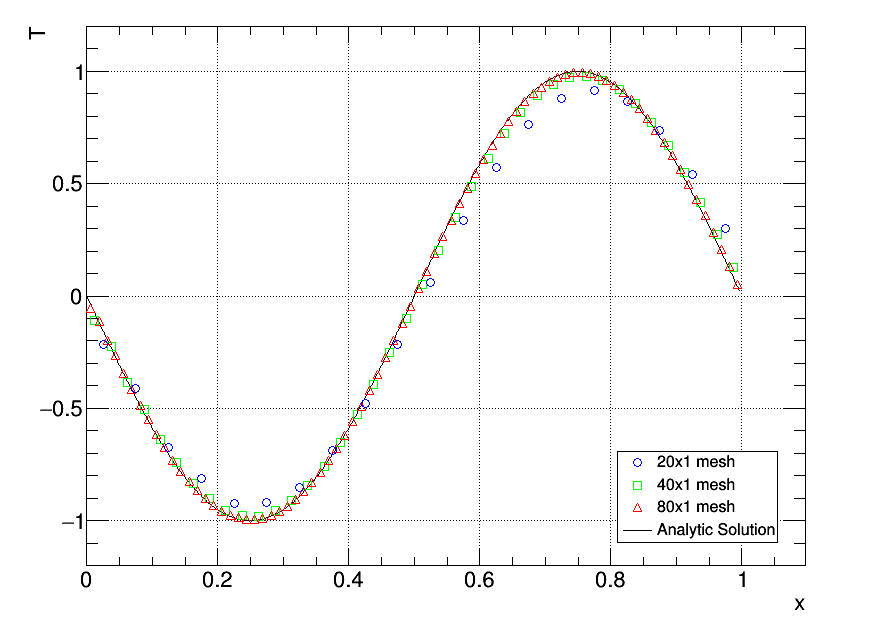
\includegraphics[width=0.85\linewidth]{qq11}
\caption{The solution at $t=1$ for mesh sizes of 20, 40, and 80}
\label{q4}
\end{figure}

The order of accuracy for the scheme was determined using the log log method as displayed in figure \ref{ord}. The order of accuracy for this scheme was estimated to be 2nd order accurate based on the $L_2$ data from 6 different meshes. This matches what was expect by implementing a 2nd order interior and boundary flux evaluation scheme.

 \begin{table}[H]
\begin{center}
    \begin{tabular}{ | p{0.13\linewidth} | p{0.2\linewidth} |p{0.1\linewidth} |p{0.1\linewidth} |p{0.1\linewidth} |}
 \hline  
     \RaggedRight \textbf{Mesh Size}
    &\RaggedRight \textbf{$L^2$norm}
    &\RaggedRight \textbf{$\triangle x$}
    &\RaggedRight \textbf{$\triangle t$}
    &\RaggedRight \textbf{Order}
    \\ \hline  
           \RaggedRight 20 x 1
    &\RaggedRight 8.158$*10^{-2}$
    &\RaggedRight 0.05
    &\RaggedRight 0.01
    &\RaggedRight -
    \\ \hline 
           \RaggedRight 40 x 1
    &\RaggedRight 2.399$*10^{-2}$
    &\RaggedRight 0.025
    &\RaggedRight 0.005
    &\RaggedRight 1.934
    \\ \hline 
           \RaggedRight 80 x 1
    &\RaggedRight 6.445$*10^{-3}$
    &\RaggedRight 0.0125
    &\RaggedRight 0.0025
    &\RaggedRight 1.937
    \\ \hline 
           \RaggedRight 160 x 1
    &\RaggedRight 1.676$*10^{-3}$
    &\RaggedRight 0.00625
    &\RaggedRight 0.00125
    &\RaggedRight 1.942
    \\ \hline 
 
    
    
    \end{tabular}
\end{center} 
\caption{Table of $L^2$ norms for increasing mesh size for $CFL = 0.4$}
\label{norm} 
\end{table}



\begin{figure}[H]
\centering
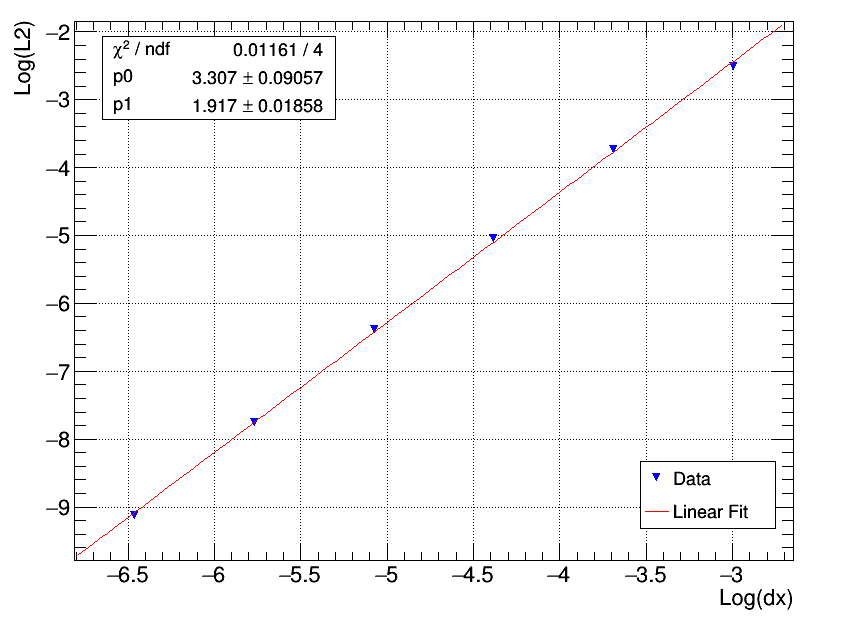
\includegraphics[width=0.85\linewidth]{order}
\caption{Calculated Order of Accuracy}
\label{ord}
\end{figure}

\begin{figure}[H]
\centering
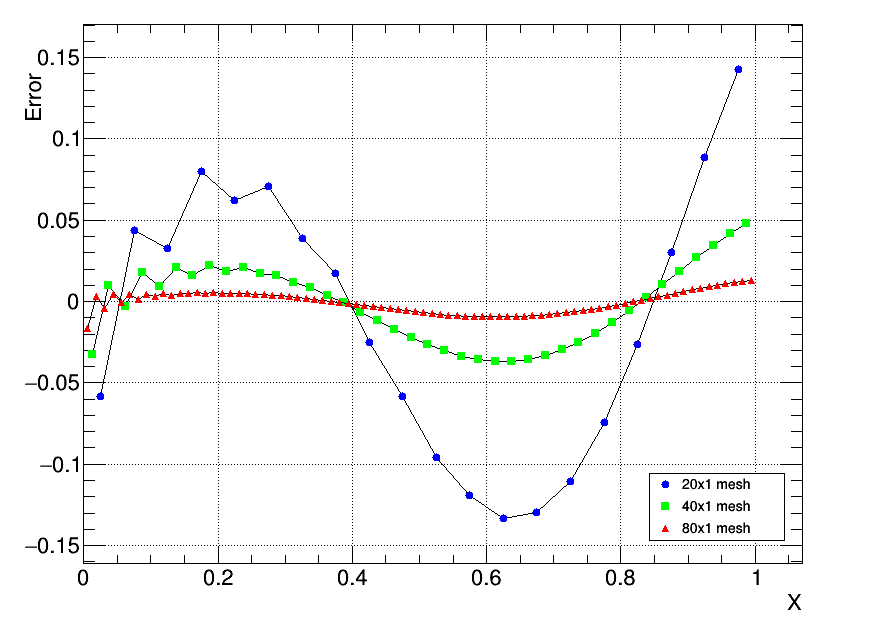
\includegraphics[width=0.85\linewidth]{qq22}
\caption{Solution Error at $t=1$ for mesh sizes of 20, 40, and 80}
\label{3D}
\end{figure}


The log-log plot enables us to estimate what mesh size would be required for a particular error. Using the plot it was found in order to obtain an error less than $10^{-3}$ a mesh size of 206.12 or greater is required. Similarly to obtain an error less than $10^{-4}$ a mesh of greater than 685.14 is required using a CFL number of 0.4.

\subsection{Stability}

\begin{figure}[H]
\centering
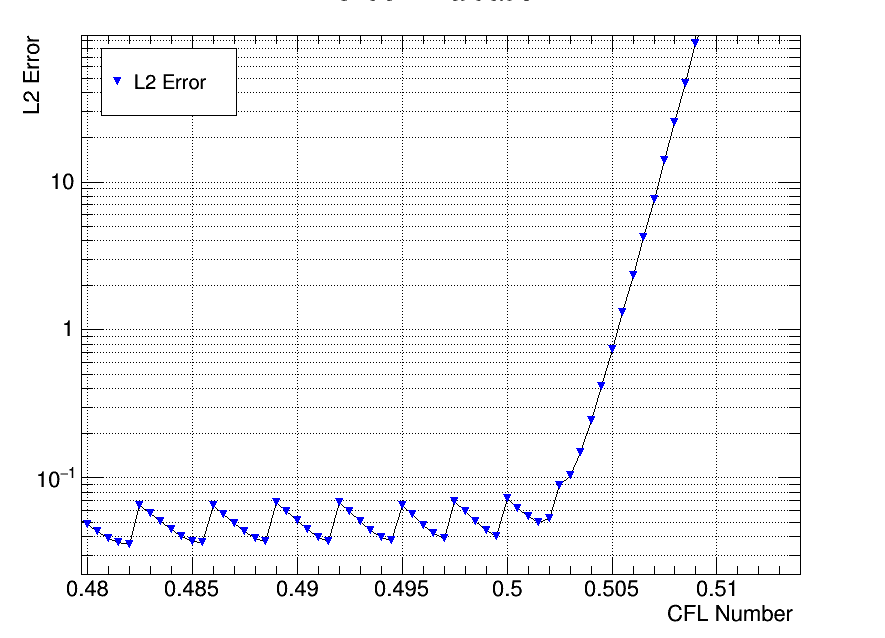
\includegraphics[width=0.85\linewidth]{stabl2}
\caption{The L2 error for increasing CFL number for a 500x1 mesh with $x_{max} = 20$}
\label{q4}
\end{figure}

\begin{figure}[H]
        \centering
        \begin{subfigure}[h]{\textwidth}
                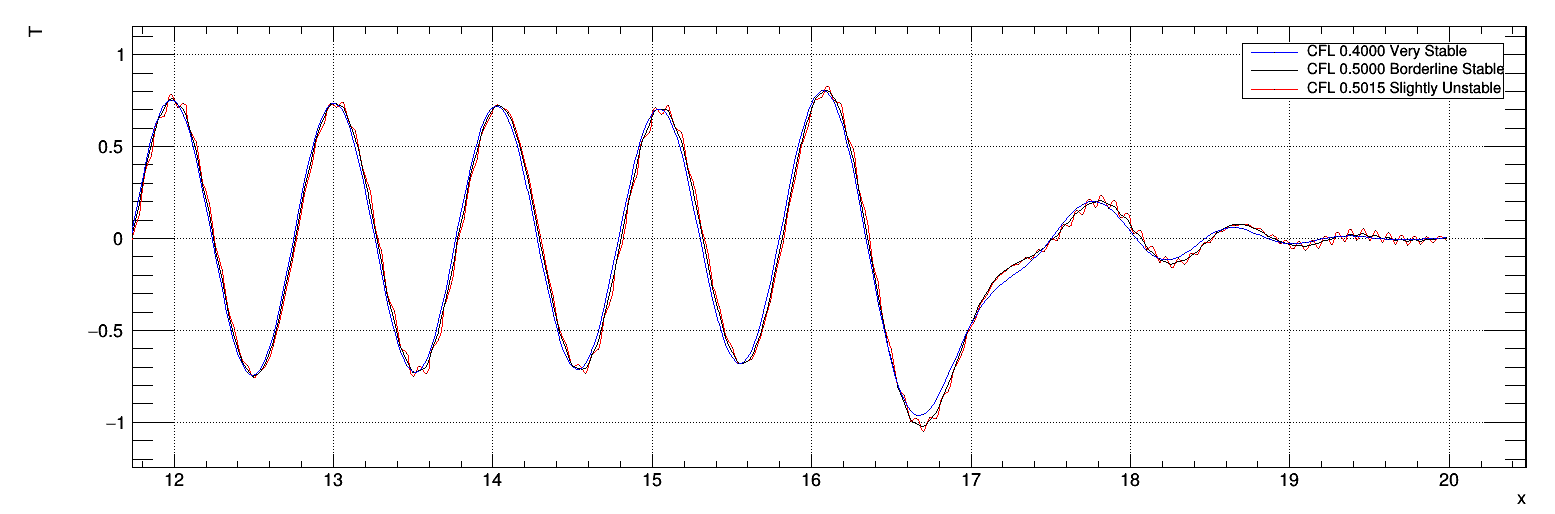
\includegraphics[width = 14.95cm]{stab1}
                \caption{}
				
        \end{subfigure}%
       ~~~~~
       
        \begin{subfigure}[h]{\textwidth}
                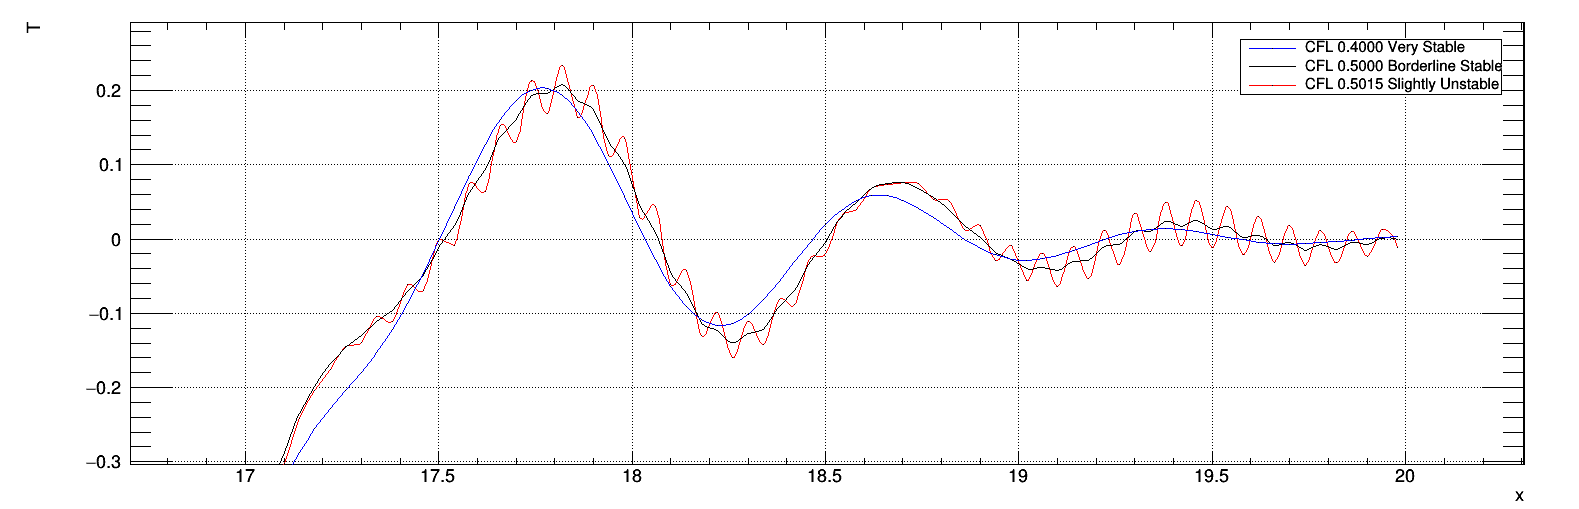
\includegraphics[width = 15.15cm]{stab3}
                \caption{}
                
        \end{subfigure}
        
        
        \begin{subfigure}[h]{\textwidth}
                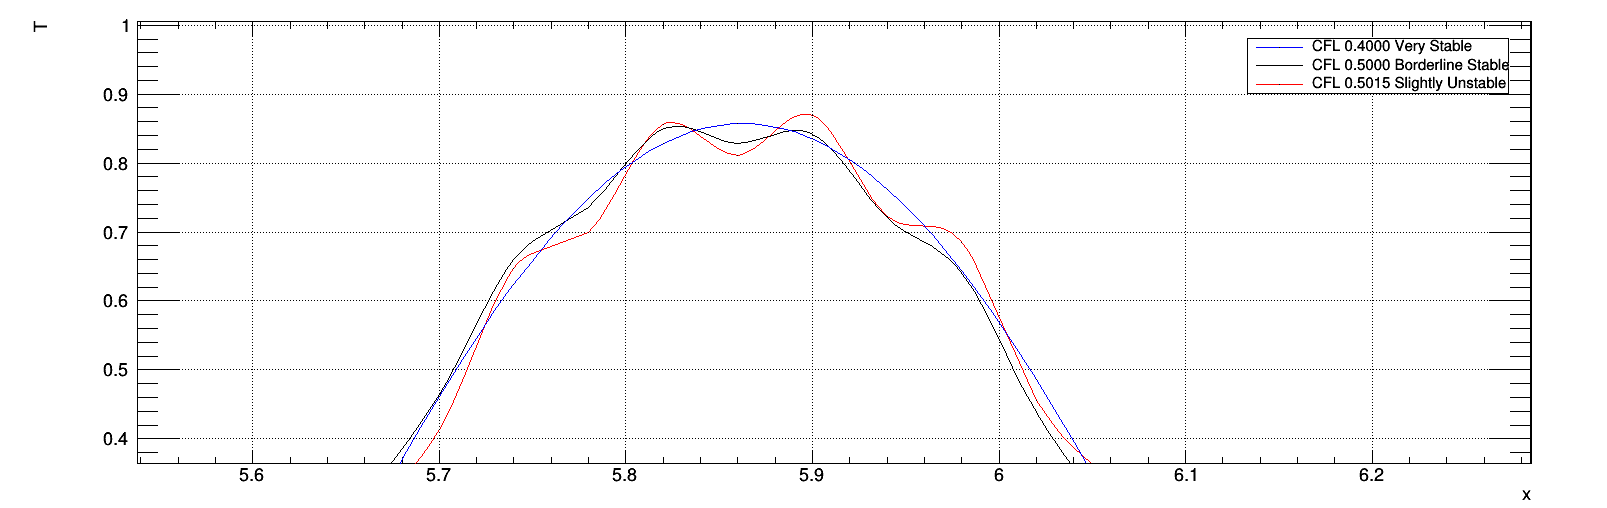
\includegraphics[width = 15.35cm]{stab2}
                \caption{}
                
        \end{subfigure}
        \caption{Maximum solution difference (a), and the $L^2$ norm of the error in converged solution (b) for $\omega = 1, 1.5$ for a 10x10 mesh }
        \label{q34}
\end{figure}


\subsection{Effect of Boundary Conditions}


\begin{figure}[H]
\centering
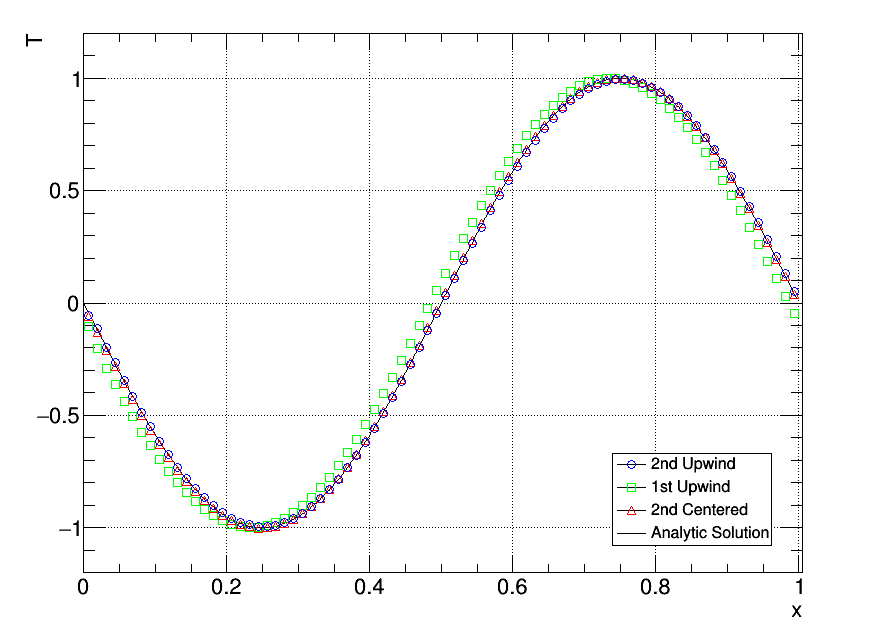
\includegraphics[width=0.8\linewidth]{3a1}
\caption{The maximum change in solution for $\omega = 1, 1.3, 1.5$ on a 20 x 20 mesh}
\label{q4}
\end{figure}

\begin{figure}[H]
\centering
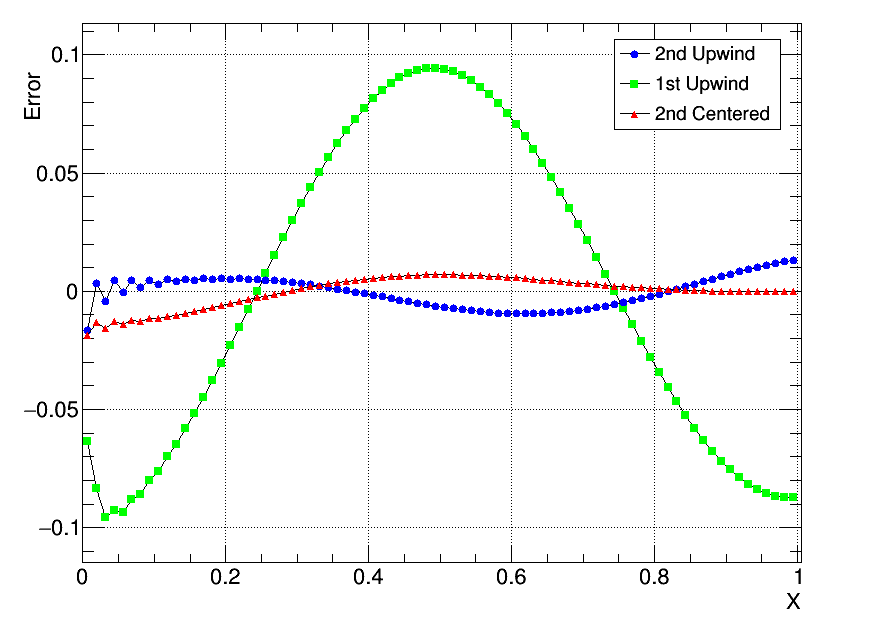
\includegraphics[width=0.8\linewidth]{3a2}
\caption{The maximum change in solution for $\omega = 1, 1.3, 1.5$ on a 20 x 20 mesh}
\label{q4}
\end{figure}

\begin{figure}[H]
\centering
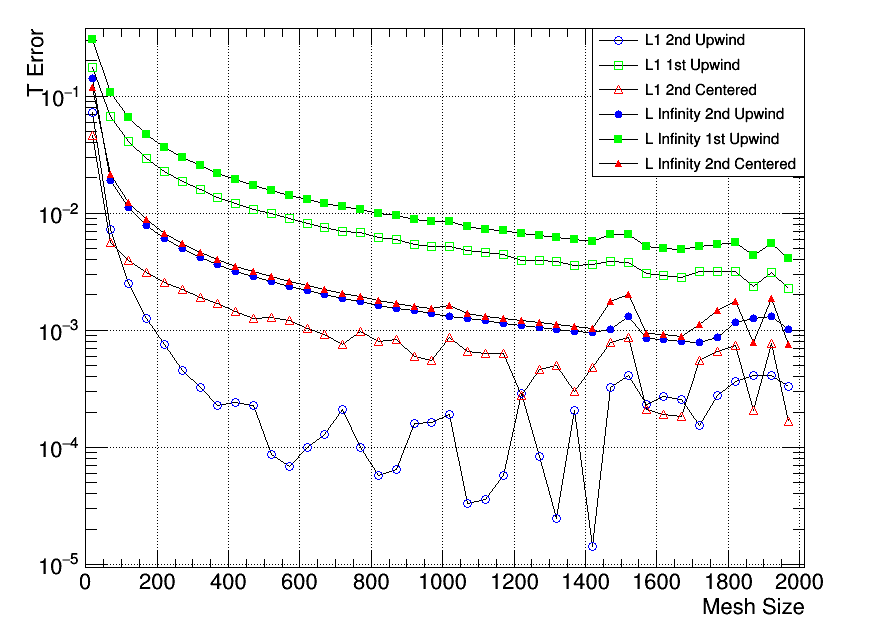
\includegraphics[width=0.8\linewidth]{3a33}
\caption{The maximum change in solution for $\omega = 1, 1.3, 1.5$ on a 20 x 20 mesh}
\label{q4}
\end{figure}




 \begin{table}[H]
\begin{center}
    \begin{tabular}{ | p{0.13\linewidth} | p{0.2\linewidth} |p{0.1\linewidth} |p{0.1\linewidth} |p{0.1\linewidth} |}
 \hline  
     \RaggedRight \textbf{Mesh Size}
    &\RaggedRight \textbf{$L^2$norm}
    &\RaggedRight \textbf{$\triangle x$}
    &\RaggedRight \textbf{Order}
    &\RaggedRight \textbf{Ratio}
    \\ \hline  
           \RaggedRight 10 x 10 
    &\RaggedRight 2.457$*10^{-3}$
    &\RaggedRight 0.1
    &\RaggedRight -
    &\RaggedRight -
    \\ \hline 
           \RaggedRight 20 x 20
    &\RaggedRight 6.384$*10^{-4}$
    &\RaggedRight 0.05
    &\RaggedRight 1.94
    &\RaggedRight 3.84
    \\ \hline 
           \RaggedRight 40 x 40
    &\RaggedRight 1.603$*10^{-4}$
    &\RaggedRight 0.025
    &\RaggedRight 1.96
    &\RaggedRight 3.98
    \\ \hline 
           \RaggedRight 80 x 80
    &\RaggedRight 3.827$*10^{-5}$
    &\RaggedRight 0.0125
    &\RaggedRight 2.00
    &\RaggedRight 4.18
    \\ \hline 
 
    
    
    \end{tabular}
\end{center} 
\caption{Table of $L^2$ norms for increasing mesh size}
\label{norm} 
\end{table}

 \begin{table}[H]
\begin{center}
    \begin{tabular}{ | p{0.1\linewidth} |p{0.2\linewidth} |p{0.1\linewidth} |}
 \hline  
    \RaggedRight \textbf{Tolerance}
    &\RaggedRight \textbf{$L^2$norm}
    &\RaggedRight \textbf{$\omega$}
    \\ \hline  
           \RaggedRight $10^{-6}$ 
    &\RaggedRight 1.767$*10^{-4}$
    &\RaggedRight 1.0
    \\ \hline 
           \RaggedRight $10^{-7}$
    &\RaggedRight 1.605$*10^{-4}$
    &\RaggedRight 1.0
    \\ \hline 
           \RaggedRight $10^{-8}$
    &\RaggedRight 1.603$*10^{-4}$
    &\RaggedRight 1.0
    \\ \hline 
           \RaggedRight $10^{-9}$
    &\RaggedRight 1.603$*10^{-4}$
    &\RaggedRight 1.0
    \\ \hline 
              \RaggedRight $10^{-10}$
    &\RaggedRight 1.603$*10^{-5}$
    &\RaggedRight 1.0
    \\ \hline 
    \RaggedRight $10^{-7}$
    &\RaggedRight 1.603872$*10^{-5}$
    &\RaggedRight 1.2
    \\ \hline 
    \RaggedRight $10^{-7}$
    &\RaggedRight 1.603879$*10^{-5}$
    &\RaggedRight 1.4
    \\ \hline 
    \RaggedRight $10^{-7}$
    &\RaggedRight 1.603896$*10^{-5}$
    &\RaggedRight 1.6
    \\ \hline 
 
    
    
    \end{tabular}
\end{center} 
\caption{Table of $L^2$ norms in relation to tolerance and over-relaxation parameter $\omega$}
\label{tol} 
\end{table}

The accuracy of the program was estimated by calculating and tabulating the $L^2$ norms of solution error for multiple mesh sizes. Using table \ref{norm} we can estimate the order of error by plotting $log(error)$ vs $log(\triangle x)$ and calculating the slope. The slope and therefore the order of accuracy was estimated to be 2.003 which rounds to 2nd order accuracy. The ratio between the errors is also indicated in table \ref{norm}, which gives us an indication of how the error is reduced relative to mesh refinement. In this case the effect of mesh refinement can be generalized in doubling the resolution we find the $L^2$ error is decrease by a quarter. Additionally as we refine the mesh se find that order converges on the order estimated by the selected estimation of solution fluxes which was 2nd order. The maximum solution change was lowered to $10^{-9}$ in order to ensure the error being measured was discretization error and not a lack of convergence. The error trend was also examined for the algorithm variables $\omega$ and the Convergence Tolerance which is displayed in table \ref{tol}. This table shows reducing the tolerance generally reduces the discretization error. 

 




\section{Poisson Problem}
\subsection{Overview}
Calculating pressure for in-compressible flows is done by solving the Poisson problem for pressure. Starting with the momentum equations one can obtain a simplified expression for Poisson problem (equation \ref{d3}). This equation allows us to simply add a source term (equation \ref{d4}) to our existing Laplace code and compute the pressure for the previous square domain as displayed in equation \ref{th}.


\begin{equation}
\label{d3}
\frac{\partial^2P}{\partial x^2} + \frac{\partial^2P}{\partial y^2} = -\Bigg(\Bigg(\frac{\partial u}{\partial x}\Bigg)^2 +2\frac{\partial v}{\partial x}\frac{\partial u}{\partial y}        +\Bigg(\frac{\partial v}{\partial y}\Bigg)^2\Bigg)
\end{equation}

\begin{equation}
\label{d4}
S_{ij} = (3x^2-3y^2)^2+2(36x^2y^2)+(3y^2-3x^2)
\end{equation}
For boundary conditions $\frac{\partial P}{\partial n}=0$ at $x=0$ and $y=0$, and $P=5-\frac{1}{2}(1+y^2)^3$ for $x=1$ and $P=5-\frac{1}{2}(1+x^2)^3$ for $y=1$ were implemented. 





 \begin{table}[H]
\begin{center}
    \begin{tabular}{ | p{0.13\linewidth} | p{0.12\linewidth}| p{0.2\linewidth} |p{0.15\linewidth} |p{0.1\linewidth} |p{0.1\linewidth} |}
 \hline  
     \RaggedRight \textbf{Mesh Size}
    &\RaggedRight \textbf{Solution}
    &\RaggedRight \textbf{Apparent Order}
    &\RaggedRight \textbf{Rel Error}
    &\RaggedRight \textbf{Extrap Value}
    &\RaggedRight \textbf{GCI}
    \\ \hline  
           \RaggedRight 10 x 10 
    &\RaggedRight 4.941434 
    &\RaggedRight -
    &\RaggedRight -
    &\RaggedRight -
    &\RaggedRight -
    \\ \hline 
           \RaggedRight 20 x 20
    &\RaggedRight 4.938539 
    &\RaggedRight -
    &\RaggedRight 0.0058\%
    &\RaggedRight -
    &\RaggedRight -
    \\ \hline 
           \RaggedRight 40 x 40
    &\RaggedRight 4.937872 
    &\RaggedRight 2.468819 
    &\RaggedRight 0.0037\%
    &\RaggedRight 4.937703
    &\RaggedRight 0.0043\%
    \\ \hline   
           \RaggedRight 80 x 80
    &\RaggedRight 4.938059
    &\RaggedRight 1.895416 
    &\RaggedRight 0.0037\%
    &\RaggedRight 4.937605
    &\RaggedRight 0.0019\% 
      \\ \hline   
           \RaggedRight 160 x 160
    &\RaggedRight 4.938802 
    &\RaggedRight 1.624394 
    &\RaggedRight 0.015\%
    &\RaggedRight 4.936539
    &\RaggedRight 0.0315\% 
    \\ \hline 
 
    
    
    \end{tabular}
\end{center} 
\caption{Table of $L^2$ norms for increasing mesh size}
\label{pnorm} 
\end{table}

Decreasing the grid size will help the solution converge closer to the exact values. If we image the grid size becoming infinitely small the grid would become continuous and essentially would describe the exact solution. However Decreasing grid size (increasing array size) has a hard hit on computational performance. Therefore before solving such a problem one should consider the exactness required for their problem and apply the appropriate mesh size. In the case where the mesh density can vary through out the problem domain it makes sense to refine the mesh in the areas of interest while providing a course mesh for areas that are understood relatively well. This will ensure the problem is solved the fastest while attaining the best approximate solution.

\section{Conclusion}
This project provides great inside to the internal algorithms used for calculating numerical solutions for symmetric grids. The Laplace problem provided a great platform for developing and testing the program. Having the analytic solution really help fine tune the program and helped given an idea on how accurate the solutions could be. Applying the program to Poisson problem showed how one could find a solution and still estimate error without a known solution to compare with. Numerical methods provide a great way of solving difficult problems and until new methods are discovered for finding exact solution will remain the main method for finding solutions to unsolvable problems. 






\appendix
\section{Appendix} \label{App:Appendix}
\subsection{Poisson.cpp}
\begin{lstlisting}
/*-------------------------------------------------------------------------------//
Main Program for finding pressure for imcompressible flows using Poisson equations.
Finds solution at P(1/2,1/2) for Land descretization error for w values of 1 for 
20x20,40x40 and 60x60 array

Jerin Roberts 2016
compiled using g++/gcc version 5.4.0 on Ubuntu 16.04.02 and are available for clone 
via the link provided: url{https://github.com/j16out/
//-------------------------------------------------------------------------------*/


#include <vector>
#include <iostream>
#include <cstdlib>
#include <fstream>
#include <string>
#include <vector>
#include <algorithm>
#include <sstream>
#include <math.h> 
#include "TApplication.h"
#include "vroot/root.hpp"
#include "numerical/numerical.hpp"

using namespace std;


#define E07 0.0000001
#define E08 0.00000001
#define E09 0.000000001
#define E10 0.0000000001
#define E11 0.00000000001




int main(int argc, char **argv)
{


carray poisson1;//my main array
carray poisson2;
carray poisson3;

//set array size or default used 162x162
set_array_size(poisson1, 20, 20, 1.0);//array, xsize, ysize, dimension
set_array_size(poisson2, 40, 40, 1.0);
set_array_size(poisson3, 80, 80, 1.0);


//set ghost cells as boundary conditions


set_zero(poisson1);
set_ghostcells(poisson1);//set ghost cells/boundaries
//print_array(poisson1);//print array in terminal


set_zero(poisson2);
set_ghostcells(poisson2);
//print_array(poisson2);

set_zero(poisson3);
set_ghostcells(poisson3);
//print_array(poisson3);



//---------------------GS SOR w=1.3 loop 1----------------------//

solve_arraySOR(poisson1, E11, 1.3);
cout << "Solution: " << get_solution(poisson1) << "\n";


//---------------------GS SOR w=1.3 loop 2----------------------//

solve_arraySOR(poisson2, E11, 1.3);
cout << "Solution: " << get_solution(poisson2) << "\n";

//---------------------GS SOR w=1 loop 3----------------------//

solve_arraySOR(poisson3, E11, 1.3);
cout << "Solution: " << get_solution(poisson3) << "\n";

//---------------------calc error based on ASME---------------//

get_discrete_Error(poisson3, poisson2, poisson1, 1.0);


//----------------------Draw Data---------------------//



if(1)//start root application
{
	TApplication theApp("App", &argc, argv);
	draw_3DgraphP(poisson3);//draw 3d graph
	theApp.Run();
}



//end
}



\end{lstlisting}
\subsection{numerical.hpp}
\begin{lstlisting}
#ifndef numerical_INCLUDED
#define numerical_INCLUDED


#include <vector>
#include <iostream>
#include <cstdlib>
#include <fstream>
#include <string>
#include <vector>
#include <algorithm>
#include <sstream>
#include <math.h> 
#include <iomanip>

using namespace std;

#define BIG 1000000
#define maxx 160
#define maxy 160
#define PI 3.141592654



struct carray{
float mcell [maxx][maxy];
vector<float> l2norm;
vector<float> diff;
int sizex = maxx;
int sizey = maxy;
int iterations = 0;
float DIM1 = 0;

};


void set_array_size(carray & myarray, int x, int y, float DIM);//set array size

void set_ghostcells(carray & myarray);//set ghost cells


void set_zero(carray & myarray);//zero entire array

void print_array(carray & myarray);//print array in terminal

float gs_iter_SOR(carray & myarray, float omega);//complete one gauss-seidel iteration with SOR

float calc_source(carray & myarray, int i, int j);//calculate source term

float calc_newcell(carray & myarray, float source, float Tip1_j, float Tim1_j, float Ti_jp1 ,float Ti_jm1);//calculate new cell value based on 2nd order scheme

void get_surcells(carray & myarray, float & Tip1_j, float & Tim1_j, float & Ti_jp1 ,float & Ti_jm1, int i, int j);//obtain values of surrounding cells

void solve_arraySOR(carray & myarray, float E0, float w);//solve the array using gs-iterations

void get_discrete_Error(carray ray1, carray ray2, carray ray3, float DIM);//get error using 3 arrays based on ASME solution accuarcy handout

float get_solution(carray & myarray);//find solution at p(1/2,1/2) for Poisson

float get_l2norm(carray & myarray, carray myarray2);//get estimated vale for l2 norm between arrays


#endif
\end{lstlisting}
\subsection{numerical.cpp}
\begin{lstlisting}
#include "numerical.hpp"





//----------set array size (working area excluding ghost)---------------//

void set_array_size(carray & myarray, int x, int y, float DIM)
{
	if(x < 160 && y < 160)
	{
	myarray.sizex = x+2;
	myarray.sizey = y+2;
	myarray.DIM1 = DIM/(x);
	}
	else
	cout << "Array size to big, setting to default 160" << "\n";

}


//--------------------------zero array----------------------------//

void set_zero(carray & myarray)
{
	for(int i = 0; i < myarray.sizex; ++i)
	{
		for(int j = 0; j < myarray.sizey; ++j)
		{
		myarray.mcell[i][j] = 0;//set everything to zero

		}
	}
}


//--------------------------set ghost cells for Poisson----------------------------//


void set_ghostcells(carray & myarray)
{
float DIM1 = myarray.DIM1;

//set boundary conditions in ghost cells
for(int i = 1; i < myarray.sizex-1; ++i)
	{float d = (i-0.5)*DIM1;
	
	//neumann boundaries	
	myarray.mcell[i][0] = myarray.mcell[i][1];//top ghost cells 
	myarray.mcell[0][i] = myarray.mcell[1][i];//left ghost cells
		
	//dirichlet boundaries	
	myarray.mcell[i][myarray.sizex-1] = 2.0*(5.0-((1.0/2.0)*pow((1.0+pow(d, 2)),3))) - myarray.mcell[i][myarray.sizex-2];
	myarray.mcell[myarray.sizey-1][i] = 2.0*(5.0-((1.0/2.0)*pow((1.0+pow(d, 2)),3))) - myarray.mcell[myarray.sizex-2][i];
	
        }
}



//--------------------------Guass-Seidel SOR----------------------------//

float gs_iter_SOR(carray & myarray, float omega)
{
float DIM1 = myarray.DIM1;//get dimensions of array (not grid size)
float Tip1_j, Tim1_j, Ti_jp1, Ti_jm1;//define values for surrounding cells
float l2sum = 0.0;
float sx = myarray.sizex-2;
float sy = myarray.sizey-2;

float dx = 0.0;//change in x
float dy = 0.0;//change in y

carray oldarray=myarray;


//-----iterate through all x for steps y -----//
set_ghostcells(myarray);

for(int j = 1; j < myarray.sizey-1; ++j)
{


	for(int i = 1; i < myarray.sizex-1; ++i)
	{
	
	dx = (i-0.5)*DIM1;
	dy = (j-0.5)*DIM1;
	
	//----get surrounding cells and compute new cell-------//
	get_surcells(myarray, Tip1_j, Tim1_j, Ti_jp1 , Ti_jm1, i, j);		
	float source = calc_source(myarray, i, j);
	float newcell = calc_newcell(myarray, source, Tip1_j, Tim1_j, Ti_jp1 , Ti_jm1); 
	
	//----apply over-relaxation-----//
	float delta = newcell - myarray.mcell[i][j];
	float newcellSOR = myarray.mcell[i][j] + omega*(delta);
	
	//-----update current cell----//
	myarray.mcell[i][j] = newcellSOR;
	

	}

}
	
set_ghostcells(myarray);	
//-----iterate through all y for steps x -----//		
for(int i = 1; i < myarray.sizey-1; ++i)
{


	for(int j = 1; j < myarray.sizex-1; ++j)
	{
	
	dx = (i-0.5)*DIM1;
	dy = (j-0.5)*DIM1;
	
	//----get surrounding cells and compute new cell-------//
	get_surcells(myarray, Tip1_j, Tim1_j, Ti_jp1 , Ti_jm1, i, j);		
	float source = calc_source(myarray, i, j);
	float newcell = calc_newcell(myarray, source, Tip1_j, Tim1_j, Ti_jp1 , Ti_jm1); 
	
	//----apply over-relaxation-----//
	float delta = newcell - myarray.mcell[i][j];
	float newcellSOR = myarray.mcell[i][j] + omega*(delta);

	
	//-----update current cell----//
	myarray.mcell[i][j] = newcellSOR;
	
	}

}


float maxdiff = -1.0;

for(int i = 2; i < myarray.sizey-2; ++i)
{	
	for(int j = 2; j < myarray.sizex-2; ++j)
	{
	float diff = abs(oldarray.mcell[i][j] - myarray.mcell[i][j]);
		if(diff > maxdiff)
		{
		maxdiff = diff;
		//cout << "coord " << maxdiff << " " << i << "  " << j << "\n";
		}
	}	

}

//for obtaining l2norm convergence

/*carray analytic;
set_array_size(analytic, 10, 10, 1.0);
set_analytic(analytic);
//float norm = get_l2norm(myarray, analytic);

myarray.l2norm.push_back(norm);	*/
myarray.diff.push_back(maxdiff);
++myarray.iterations; 

return maxdiff;
}
//-------------------------Get L2 nrom for unknown analytical----------------------//

float get_l2norm(carray & myarray, carray myarray2)
{
float l2sum =0;
float sx = myarray.sizex-2;
float sy = myarray.sizey-2;

for(int j = 1; j < myarray.sizey-1; ++j)
{	
	for(int i = 1; i < myarray.sizex-1; ++i)
	{

	float P = myarray.mcell[i][j];
	float T = myarray2.mcell[i][j];
	l2sum =  l2sum + pow((P-T),2);

	}

}

float l2 = sqrt(l2sum/(sx*sy));
cout << "L2 norm: " << l2 << "\n";
return l2;
}

//--------------------------Solve array using GS-iterations----------------------------//

void solve_arraySOR(carray & myarray, float E0, float w)
{
printf("\n\nSolving Grid size: %d Relaxation: %f\n", myarray.sizex, w);
bool relax_on = true; 
float diff = 1;// current difference
float ldiff = BIG;// previous difference
int div = 0;
int update = 0;
int update2 = 100;

while(diff >= E0)
{
diff = gs_iter_SOR(myarray, w);


	if(diff > BIG)//avoid infinite loops if diverges
	break;

	if(update >= update2)//report difference every 100 steps
	{cout << "Update: step " << update << " Solution Change: " << setprecision(9) << fixed << diff << " \n"; 
	//print_array(myarray);
	 update2 = update2 + 100;
	}
	
	if(ldiff == diff)//checks for repeated values indication of instability for high w
	++div;
	else
	div = 0;

	if(div > 3 && w > 1.1)//reduces over-relaxation for high w when unstable
	{
	w = 1.0;
	cout << "Relaxation Reduced to "<<w<<" @ " << myarray.iterations << " \n";
	}
		
ldiff = diff;
++update;	
}

cout << "Iterations: " << myarray.iterations <<  "\n";
}


//--------------------------Print array in terminal----------------------------//

void print_array(carray & myarray)
{
cout << "\n";

	for(int j = 0; j < myarray.sizey; ++j)
	{
	cout << "\n|";	
		for(int i = 0; i < myarray.sizex; ++i)
		{
		if(myarray.mcell[i][j] >= 0)
		cout << setprecision(3) << fixed << myarray.mcell[i][j] <<"|";
		if(myarray.mcell[i][j] < 0)
		cout << setprecision(2) << fixed << myarray.mcell[i][j] <<"|";
		}
	
	}
cout << "\n";
}

//--------------------Calculate new cell value from neighbors ---------------------//


float calc_newcell(carray & myarray, float source, float Tip1_j, float Tim1_j, float Ti_jp1 ,float Ti_jm1)
{
float DIM1 = myarray.DIM1;
float chx = DIM1;
float chy = DIM1;
float temp = (pow(chx,2)*pow(chy,2)) /  (2*(pow(chx,2)+pow(chy,2)));
float newcell = ((  ((Tip1_j+Tim1_j)/pow(chx,2))  +  ((Ti_jp1+Ti_jm1)/pow(chy,2)) - source ) * temp) ;

return newcell;
}
//---------------------Get source term for poisson problem----------------------//
float calc_source(carray & myarray, int i, int j)
{
float DIM1 = myarray.DIM1;
float dx = (i-0.5)*DIM1;
float dy = (j-0.5)*DIM1;
float source = -1.0*(pow(3*pow(dx,2)-3*pow(dy,2),2)+72.0*(pow(dx,2)*pow(dy,2))+pow(3*pow(dy,2)-3.0*pow(dx,2),2));
//source = 0 for Laplace problem

return source;
}

//-----------------------Get average solution at point (1/2)(1/2)--------------------//

float get_solution(carray & myarray)
{
float DIM1 = myarray.DIM1;
int sx = (myarray.sizex)/2.0;
int sy = (myarray.sizey)/2.0;
float sol = (myarray.mcell[sx-1][sy]+myarray.mcell[sx][sy]+myarray.mcell[sx][sy-1]+myarray.mcell[sx-1][sy-1])/4.0;

printf("cell 1: %f cell 2: %f cell 3: %f cell 4: %f\n",myarray.mcell[sx-1][sy],myarray.mcell[sx][sy],myarray.mcell[sx][sy-1],myarray.mcell[sx-1][sy-1]);
//for Poisson problem only, finds value based on average of four surrounding cells

return sol;
}

//--------------------------Get current cell values----------------------------//

void get_surcells(carray & myarray, float & Tip1_j, float & Tim1_j, float & Ti_jp1 ,float & Ti_jm1, int i, int j)
{
float fcon = false;
float sizex = myarray.sizex;
float sizey = myarray.sizey;

		Tip1_j = myarray.mcell[i+1][j];
		Tim1_j = myarray.mcell[i-1][j];
		Ti_jp1 = myarray.mcell[i][j+1];
		Ti_jm1 = myarray.mcell[i][j-1];

}

//--------------------------Get descrete error----------------------------//

void get_discrete_Error(carray ray1, carray ray2, carray ray3, float DIM)
{
//Calculating error as described in paper "procedure for estimation and reporting of uncertainty due to discretization in CFD applications"//

printf("\nCalculating Error...\n");

float h1 = DIM/ray1.sizex;
float h2 = DIM/ray2.sizex;
float h3 = DIM/ray3.sizex;


float sol1 = get_solution(ray1);
float sol2 = get_solution(ray2);
float sol3 = get_solution(ray3);



printf("h1: %f \nh2: %f \nh3: %f, \nsol1: %f \nsol2: %f \nsol3: %f\n",h1, h2, h3, sol1, sol2, sol3);

float r21 = h2/h1;
float r32 = h3/h2;

printf("\nr32: %f \nr21: %f\n",r32, r21);

float e32 = sol3-sol2;
float e21 = sol2-sol1;

float s = (e32/e21);
if(s >= 0)
s = 1;
else
s = -1;

float p_n = 0;
float p = (1/log(r21))*(abs(log(abs(e32/e21))+0));

printf("intial guess: %f \n", p);

float diff = 1;

	while(diff > 0.0000001)
	{

	float p_n = (1/log(r21))*(abs(log(abs(e32/e21))+log((pow(r21,p)-s)/(pow(r32,p)-s)) ));
	diff = abs(p_n -p);
	//printf("p_n: %f p: %f diff: %f\n",p_n, p, diff);

	p = p_n;
	}
 
//
float sol_ext21 = (pow(r21, p)*sol1-sol2)/(pow(r21,p)-1.0);
float sol_ext32 = (pow(r32, p)*sol2-sol3)/(pow(r32,p)-1.0);

printf("order: %f \nphi_ext21: %f \nphi_ext32 %f\n",p, sol_ext21, sol_ext32);

float ea21 = abs((sol1-sol2)/sol1);

float e_ext21 = abs((sol_ext21-sol1)/sol_ext21);

float GCI_21 = (1.25*ea21)/(pow(r21,p)-1.0);


printf("ea21: %f  \ne_ext21: %f  \nGC121 %f \n", ea21, e_ext21, GCI_21);

}


\end{lstlisting}

\begin{thebibliography}{99} % Beamer does not support BibTeX so references must be inserted manually as below
\bibitem[Celik, 2006]{p0}Ismail B. Celik1, Urmila Ghia, Patrick J.Roache and Christopher J. Freitas
\newblock "Procedure for Esitmation and Reporting Uncertainty Due to Discretization in CFD apllications",  West Virginia University, Morgantown WV, USA

\end{thebibliography}


%%% End document
\end{document}